\section{Objectives and specification mapping}
Lab 11 (PDF pages 44--51) requests wire-RC analysis, driver sizing, wire-length sweeps and adjacent-wire coupling comparisons. This implementation retains the handout's three wire-parameter sets and corresponding device W/L dimensions: 45 driver-size cases, 30 length cases and 180 coupling cases, totaling three netlists and 255 completed cases.

The handout labels these sets as 0.35/0.25/0.18 $\mu$m processes at 3.3/2.5/1.8 V. The corresponding three MOS process models are unavailable. Here A/B/C identify RC and geometry scenarios; every scenario uses the same supplied model at 1 V. The results compare wire and sizing effects, and do not reproduce absolute delays for three foundry processes.

\section{Circuit, parameters and hand calculations}
The handout's three-section $\pi$ model uses three resistors $R/3$, endpoint capacitors $C/6$ and two interior capacitors $C/3$, preserving total resistance and capacitance. Inv1 drives the wire and Inv2 is the receiver. Delays $t_1$ and $t_2$ reach the driver output and receiver input with inversion; $t_3$ reaches the receiver output with the same polarity as the original input.

The 10 mm wire values from Table 11.1 and recalculated RC products are below. Set A's printed 3.17 ns is inconsistent with $1.7\times2.11=3.587$ ns. The simulation retains the R and C columns and uses their actual product; the printed value is not treated as a measurement.

\begin{center}\small
\begin{tabular}{lllll}
\toprule
Set & R (k$\Omega$) & C (pF) & RC (ns) & $W_p/W_n/L$ ($\mu$m) \\
\midrule
A & 1.70 & 2.11 & 3.587 & 2.7 / 0.9 / 0.35 \\
B & 2.38 & 2.39 & 5.688 & 1.8 / 0.6 / 0.25 \\
C & 3.39 & 2.46 & 8.339 & 1.5 / 0.5 / 0.18 \\
\bottomrule
\end{tabular}
\end{center}
Driver widths scale by N=1--15 while receiver widths stay at one unit. The length sweep fixes N=5 and covers 1--10 mm in 1 mm increments. Both wire R and C scale with length, so the internal wire-RC contribution grows approximately quadratically.

The coupling model contains left, center and right wires, with the center as victim. Every section retains both ground and interwire capacitances. Table 11.4 parameters per micrometer are:
\begin{center}\small
\begin{tabular}{lllll}
\toprule
Set & R ($\Omega/\mu$m) & $C_c$ (fF/$\mu$m) & $C_g$ (fF/$\mu$m) & $C_s$ (fF/$\mu$m) \\
\midrule
A & .17 & .08 & .07 & .14 \\
B & .24 & .09 & .05 & .14 \\
C & .34 & .10 & .04 & .14 \\
\bottomrule
\end{tabular}
\end{center}
For each scenario, victim rise/fall, six neighbor patterns R/R, R/static, R/F, static/static, static/F and F/F, and lengths 2/4/6/8/10 mm form the full $3\times2\times6\times5=180$-case matrix. Static neighboring inputs remain at 0 V. R/F describe transitions at the original input of each wire's driver.
\section{Simulation setup and measurement definitions}
The separately supplied MOS model is evaluated at 1.0 V and $27\,^{\circ}$C, retaining the handout topology and the comparison conditions below. One volt is a simulation setting, not a device rating established by available model documentation. Numerical results from the handout's older processes are not acceptance targets for this model.

HSPICE S-2021.09 runs with RUNLVL=6. Tables use actual native measurements and figures use actual printed numerical traces. Every variant resets all swept parameters and temperature, avoiding inherited settings from an earlier variant. Completed solutions and measurements do not establish process reliability. Internal warnings in encrypted model blocks remain incompletely visible.
Uncoupled tests use 100 ps input ramps, a 180 ns transient and 20 ps printing, including both polarities. Coupling tests apply a single 100 ps ramp at 20 ns and run to 120 ns. Delay is the difference between original-input and receiver-output 50\% crossings. The long observation window accommodates the slowest wire transitions.

\section{Driver-size and length results}
Larger drivers improve near-end delay, while far-end delay increasingly reaches the limit imposed by the wire itself.

\begin{figure}[htbp]
\centering
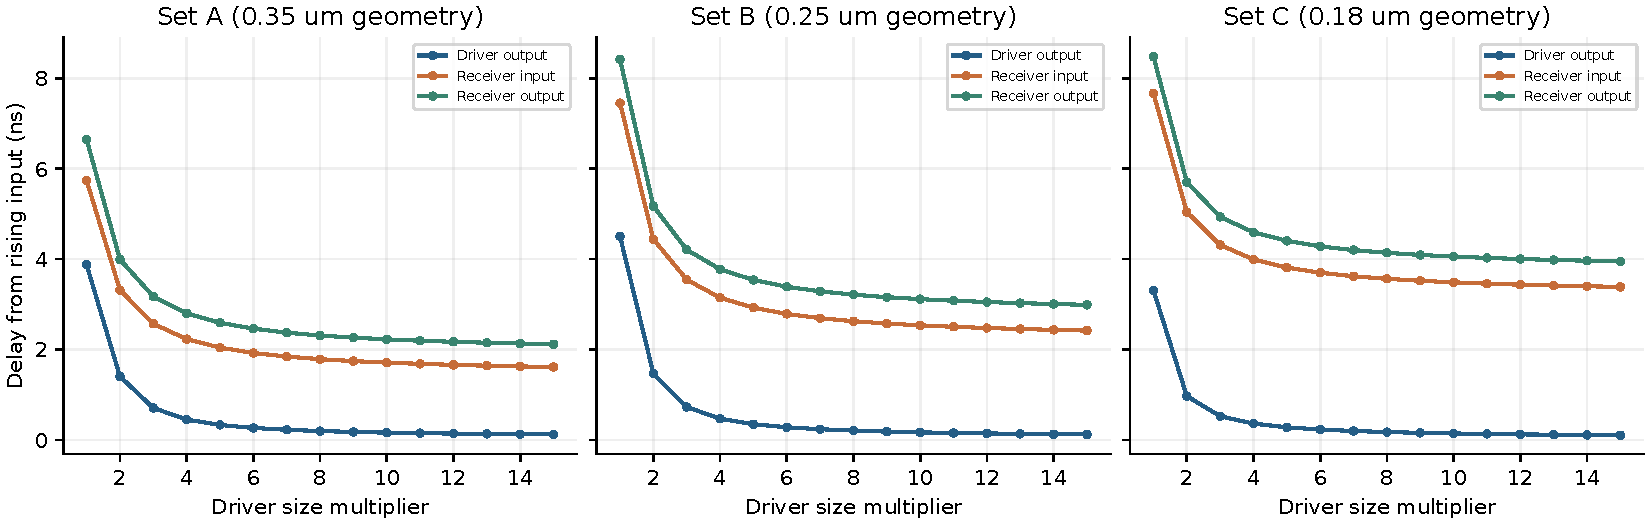
\includegraphics[width=\linewidth]{figures/wire_driver_sizing.pdf}
\caption{Three observation points on 10 mm wires; curves use the rising original input.}
\end{figure}
\begin{figure}[htbp]
\centering
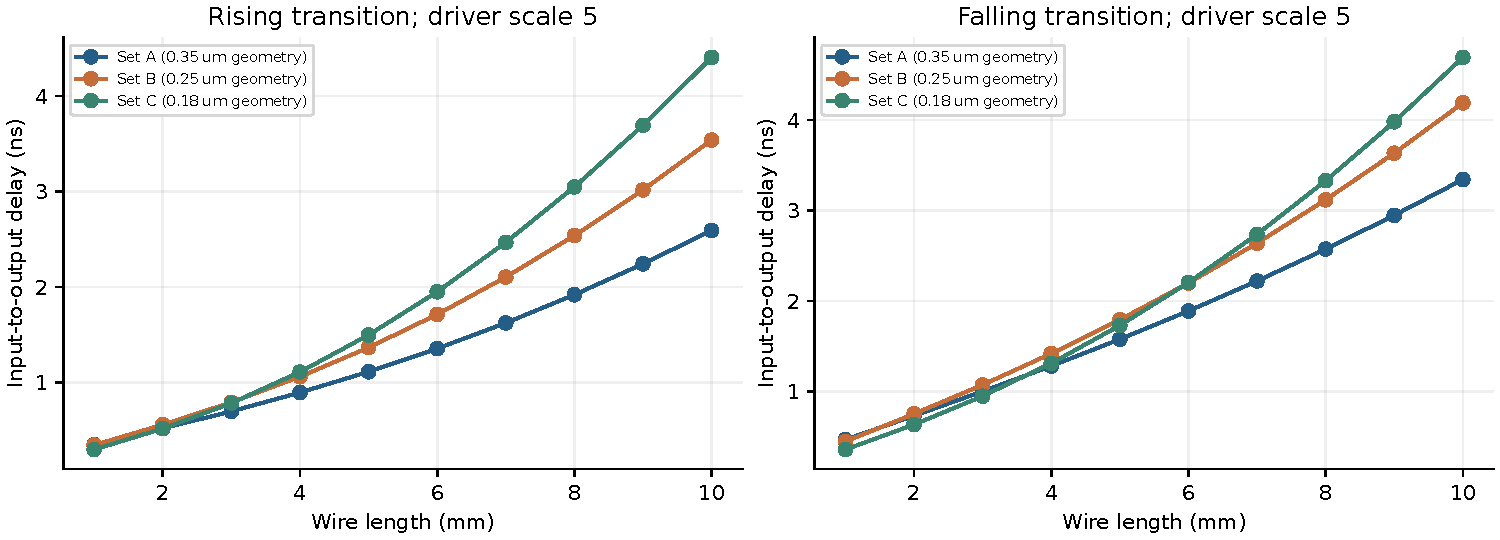
\includegraphics[width=\linewidth]{figures/wire_length.pdf}
\caption{Receiver-output delay versus wire length at N=5 for both polarities.}
\end{figure}
\begin{center}\small
\begin{tabular}{llll}
\toprule
Set & N=1, $t_3$ (ns) & N=5, $t_3$ (ns) & N=15, $t_3$ (ns) \\
\midrule
A & 6.646 & 2.591 & 2.118 \\
B & 8.417 & 3.537 & 2.989 \\
C & 8.476 & 4.403 & 3.950 \\
\bottomrule
\end{tabular}
\end{center}
\section{Coupling results}
The table compares the 10 mm extremes of both neighbors switching with the victim or against it. Every value is from the current simulations.

\begin{center}\small
\begin{tabular}{lllll}
\toprule
Set & Victim & Same (ns) & Opposite (ns) & Ratio \\
\midrule
A & R & 1.186 & 3.978 & 3.35 \\
A & F & 1.576 & 6.064 & 3.85 \\
B & R & 1.278 & 5.477 & 4.29 \\
B & F & 1.549 & 6.990 & 4.51 \\
C & R & 1.464 & 7.424 & 5.07 \\
C & F & 1.588 & 8.069 & 5.08 \\
\bottomrule
\end{tabular}
\end{center}
\begin{figure}[htbp]
\centering
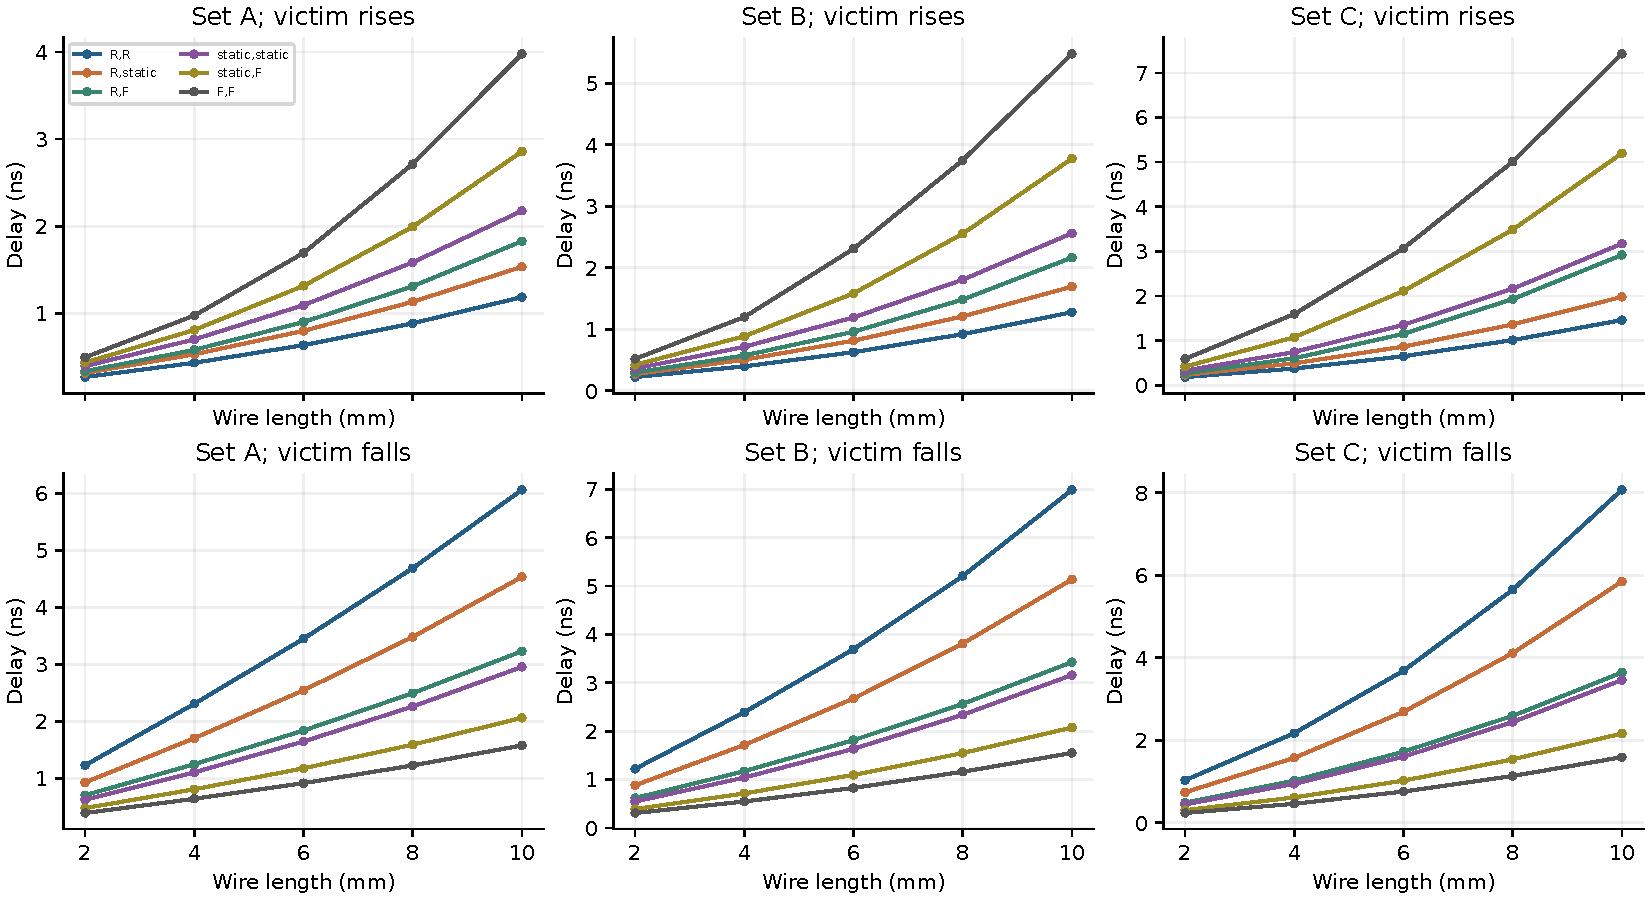
\includegraphics[width=\linewidth]{figures/wire_coupling.pdf}
\caption{All six neighbor patterns; R/F/static are defined at the driver inputs.}
\end{figure}
\section{Discussion and questions}
When adjacent wires move together, the interwire capacitor sees a smaller differential change; opposite transitions increase that change and the effective load. For ideal synchronized ramps, $C_{eff}=C_g+\sum C_c(1-dV_{adj}/dV_{victim})$, so each neighbor contributes approximately 0, $C_c$ or $2C_c$ for same-direction, static or opposite-direction motion. Real slopes and timing differ, so delay ratios need not equal these capacitance ratios.

Lower-resistivity metal, thicker or wider wires, lower-permittivity dielectrics, increased spacing and shorter routes can reduce wire delay, with tradeoffs in area, capacitance and routing resources. Circuit options include appropriately sized repeaters and tapered drivers. Oversizing only the first driver loads its predecessor and cannot remove the wire's intrinsic RC. Shielding reduces crosstalk but adds ground capacitance and consumes metal resources.

All RC and coupling scan conditions are complete. Absolute comparisons across actual fabrication processes remain limited by missing matching MOS models. Discontinuous early numbers in the handout Table 11.5(c) are not adopted as validation targets.

\section{Reproducibility files}
The following netlists accompany this report. A comment marks the local model setup; neither the model file nor its path is published. A valid local model configuration must be supplied before execution.
\begin{itemize}
\item \texttt{01\_driver\_sizing.sp}
\item \texttt{02\_wire\_length.sp}
\item \texttt{03\_coupled\_wires.sp}
\end{itemize}
The lab results directory contains every case measurement, representative waveform CSV files, derived metrics and a specification manifest. Waveform exports retain at most 2501 uniformly selected samples; direct measurements are not downsampled. Complete original listings remain local.

